\documentclass[addpoints,12pt]{exam}
\newcommand{\ds}{\displaystyle}
\usepackage[margin=0.8in]{geometry}
\usepackage{subcaption}
\usepackage{tikz}
\usepackage{amssymb,amsmath,graphicx,wrapfig,verbatim,wasysym, enumitem,psfragx,color}
\usepackage{multicol}

%\usepackage{fancyhdr}
%\setlength{\headheight}{13.6pt}
%\pagestyle{fancy}
%\lhead{Math 222}
%\chead{ Midterm 1 }
%\rhead{Spring 2022}

\def\FillInBlank{\rule{3truein} {.01truein}}




% Choose one option (bubbles)
\newcommand{\chooseone}{{\Large$\Circle$\ \ }}
% Choose multiple options (squares)
\newcommand{\choosemany}{{\Large$\Square$\ \ }}


\newcommand{\myleft}{\makebox[.4\textwidth]{First Name:\enspace\hrulefill}}
\newcommand{\myright}{\makebox[.4\textwidth]{Last Name:\enspace\hrulefill}}
\header{\oddeven{\myleft}{}}
    {}
    {\oddeven{\myright}{}}

\footrule

\footer{Math 211}
     {Midterm 2 - Practice Exam}
     {Page \thepage\ of \numpages}

\begin{document}

\begin{questions}


\question Clearly mark the correct answer(s) for each of the following by completely filling in the
appropriate bubble. \textbf{No justification is needed.}


\begin{parts}


\part[2] \textbf{(Multiple Choice-Choose one)} Suppose a rich aunt wants to buy you a car when
you get your driver's license. How much money must she deposit in a trust fund paying $4\%$
interest compounded quarterly at the time of your birth to yield $\$30,000$ on your 16th
birthday?

\begin{itemize} [label={}]
\item \chooseone $30000(1.01)^{64}$\smallskip
\item \chooseone $\dfrac{30000}{(1.01)^{64}}$\smallskip
\item \chooseone $\dfrac{30000}{(1.04)^{16}}$\smallskip
\item \chooseone $\dfrac{30000}{(1.01)^{16}}$\smallskip
\item \chooseone None of the above.
\end{itemize}

\vfill




\part[2] \textbf{(Multiple Choice-Choose one)} A store expects to sell 8000 bottles of perfume
this year. The perfume costs the store owner $\$20$ per bottle, there is an ordering fee of
$\$100$ per shipment, and the cost of storing the perfume is $\$10$ per bottle per year. The
perfume is consumed at a constant rate throughout the year, and each shipment arrives just as
the preceding shipment is used up. Which of the following is the correct expression for the
yearly \textbf{storage costs} (in dollars) of the perfume with lot size $x$? (hint: average
inventory is $x/2$).

\begin{itemize}[label={}]
\item \chooseone $5x$
\item \chooseone $5x+100$
\item \chooseone $25x+100$
\item \chooseone $(20x+100)\dfrac{8000}{x}$
\item \chooseone None of the above.
\end{itemize}

\vfill




\part[2] \textbf{(Multiple Choice-Choose one)} Suppose monthly global data traffic is predicted to
be
$2.7e^{0.475x}$ petabytes, where $x$ is the number of years since 2016. Find the relative
growth rate (per year) in 2026.
\begin{itemize}[label={}]
\item \chooseone $2.7\%$
\item \chooseone $47.5\%$
\item \chooseone $2.7e^{47.5}$
\item \chooseone None of the above.
\end{itemize}


\vfill




%\part[2] For $y=5x^2$, the differential $dy$ at $x=2$ and $dx=0.3$ is $dy=6$.
%\begin{itemize}[label={}]
%\item \chooseone True
%\item \chooseone False
%\end{itemize}

%\vfill
\newpage

\part[2] \textbf{(Choose all that apply)} Given the graph of $y=f(x)$ below, where is $f(x)$
nondifferentiable?
\begin{itemize}[label={}]
\item \choosemany $x=-1$

\item \choosemany $x=0$
\item \choosemany $x=1$
\item \choosemany $x=2$
\item \choosemany $x=3$
\item \choosemany None of the above.
\end{itemize}

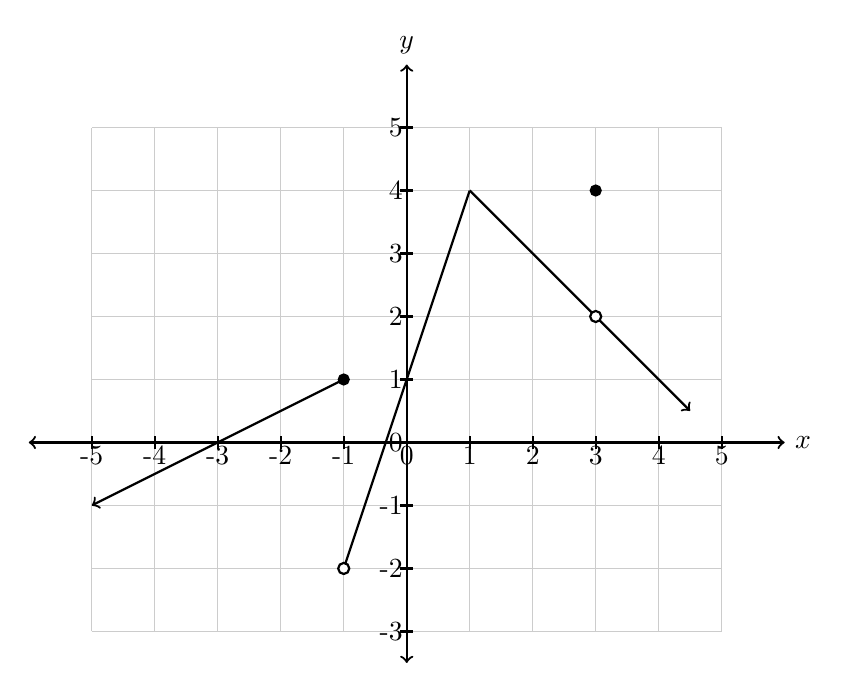
\begin{tikzpicture}[scale=.8]
\draw[gray!40] (-5, -3) grid[step=1] (5, 5);
\draw[<->,thick,black] (-6,0)--(6,0) node[right]{$x$};
\draw[<->, thick,black] (0,-3.5)--(0,6) node[above]{$y$};
\foreach \x in {-5,-4,...,5}
\draw[thick] (\x,-.1) --(\x,.1) node[below]{\x};
\foreach \y in {-3,-2,...,5}
\draw[thick] (-.1,\y) --(.1,\y) node[left] {\y};
\draw[domain=1:4.5,samples=100, thick,->] plot ({\x},{-(\x+1)+6});
\draw[domain=-1:1,samples=100, thick,-] plot ({\x},{3*\x+1});
\draw[domain=-5:-1,samples=100,thick,<-] plot ({\x},{(\x/2+1.5});
\draw[fill=black] (3,4) circle[radius=0.25em];
\draw[fill=black] (-1,1) circle[radius=0.25em];
\draw[fill=white,thick] (3,2) circle[radius=0.25em];
\draw[fill=white,thick] (-1,-2) circle[radius=0.25em];
\end{tikzpicture}




\vfill




\part[2] \textbf{(True/False)} $f(x)=e^{x^2-x}$ has a critical number at $x=0$.

\begin{itemize}[label={}]
\item \chooseone True
\item \chooseone False
\end{itemize}

\vfill

\part[2] \textbf{(True/False)} A Hyundai Sonata lists for $\$ 22,000$ and depreciates in value by
$30\%$ each year. In 3 years, it will be worth $22,000(.3)^3$.

\begin{itemize}[label={}]

\item \chooseone True
\item \chooseone False
\end{itemize}

\vfill


\end{parts}

\newpage

\question For the demand function $D(p)=40-p$:
\begin{parts}
 \part[4] Find the elasticity of demand $E(p)$ and evaluate it at $p=10.$ Simplify your answer.

 \vfill

 \part[3] Is the demand elastic or inelastic at $p=10$? To increase revenue, should you increase
or decrease the price?
   \vfill

  \part[3] Find the price at which the demand is unit-elastic.
   \vfill

\end{parts}

\newpage


\question
Suppose $f(x)$ is a continuous function whose derivative is $f'(x)=x^{-1/3}(2-x)(x+4)^2$.
\begin{parts}
\part[4] What are the critical numbers of $f(x)$?
\vspace{2in}
\part[7] At what points, if any, does $f(x)$ assume relative maximum and minimum values?
Fully justify your answer.
\end{parts}

\newpage


\question[11] On the axes below,
draw the graph of a function $f(x)$ which is continuous everywhere except $x=1$ that satisfies
the following conditions:

$f(0)=1$

$f(x)$ has a vertical asymptote at $x=1$

$f'(x)<0$ on $(4,\infty)$

$f'(x)>0$ on $(-\infty, 1)\cup(1,4)$

$f''(x)>0$ on $(-\infty, 1)$

$f''(x)<0$ on $( 1,\infty)$


        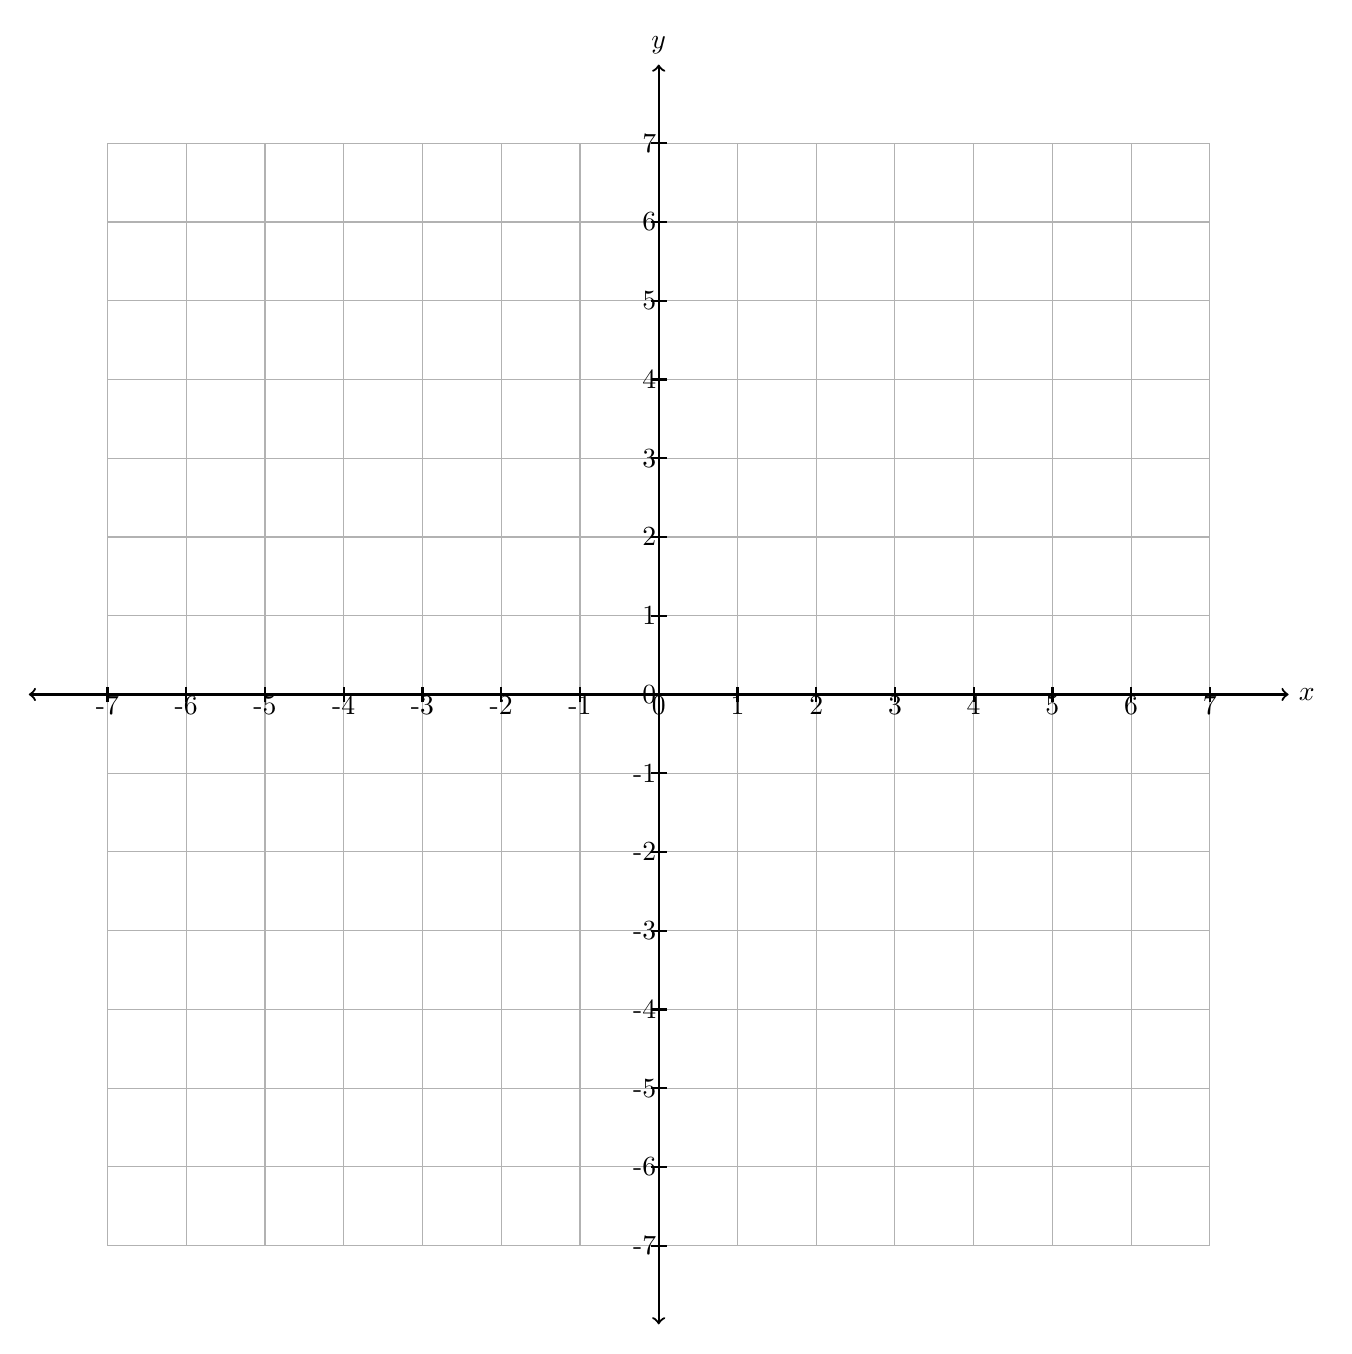
\begin{tikzpicture}[scale=1]
        \draw[gray!60] (-7, -7) grid[step=1] (7, 7);
        \draw[<->, thick,black] (-8,0)--(8,0) node[right]{$x$};
        \draw[<->, thick,black] (0,-8)--(0,8) node[above]{$y$};
        \foreach \x in {-7,-6,...,7}
        \draw[thick] (\x,-.1) --(\x,.1)node[below]{\x};
        \foreach \y in {-7,-6,...,7}
        \draw[thick] (-.1,\y) --(.1,\y)node[left]{\y};
        \end{tikzpicture}



\newpage

\question[12]
        A rectangular sheep pen is to be enclosed by a wooden fence and divided into two
equal parts by a chain link fence parallel to one of the sides. The wooden fencing will cost $\$4$
per foot, while the chain link will cost $\$ 2 $ per foot. With $\$400$ to spend, what dimensions
for the outer rectangle will create the largest total area? Justify your solution is optimal.

\bigskip

        \begin{figure}[h]
               \begin{center}
                      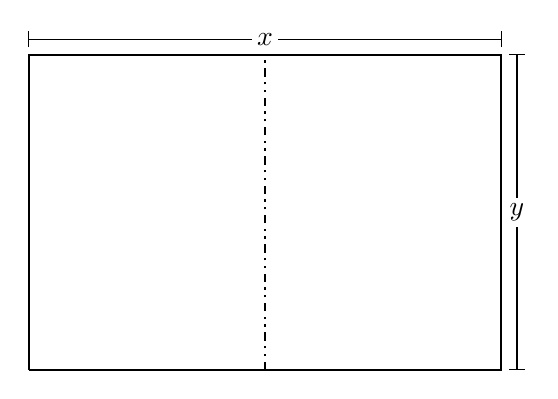
\begin{tikzpicture}
                             \draw[thick] (0,0) -- (6,0)--(6,4)--(0,4)--(0,0);
                             \draw[thick, dashdotdotted] (3,0) --(3,4);
    \draw (0,4.2)--(6,4.2);

   \draw (0,4.1)--(0,4.3);
   \draw (6,4.1)--(6,4.3);
   \draw (6.2,0)--(6.2,4);
   \draw (6.1,0)--(6.3,0);
   \draw (6.1,4)--(6.3,4);
\draw (3,4.2) node[inner sep=2pt,fill=white] {$x$};
\draw (6.2,2) node[inner sep=2pt,fill=white] {$y$};
                     
                     
                     \end{tikzpicture}
              \end{center}
              %\caption{Useful figure for Problem 4}
       \end{figure}

\newpage

\question For $f(x)=x^4-4x^3+10 $:

\begin{parts}

\part[5] Find the intervals of increasing/decreasing. Give your answers using interval notation.
Show all work.

\vfill
\part[5] Find the intervals of concave up/concave down. Give your answers using interval
notation. Show all work.
\vfill
\end{parts}

\newpage




\question[12] A bus company will rent a bus that holds 50 people to groups of 30 people or
more. If a group contains exactly 30 people, each person pays $\$80$. In large groups,
everybody's fare is reduced by $\$2$ for each person in excess of 30. Determine the size of the
group for which the bus company's revenue will be greatest. Justify why your solution is optimal.




\newpage

\question[10] Find the absolute maximum and absolute minimum of $g(x)=6x^2-x^3-6$ on
$[-1,3]$.


\vfill




\newpage

\question

\begin{parts}

\part[6] Find $f'(x)$ if $f(x) = \ln(x^2+2x)$. You do not need to simplify your final answer.

\vfill

\part[6] Find $g'(x)$ if $g(x)=e^{x^2+4x}$. You do not need to simplify your final answer.

\vfill

\end{parts}




\newpage

\end{questions}

\end{document}
